\documentclass{Beamer}
\usetheme{default}

\usepackage{polski}
\usepackage[utf8x]{inputenc}
\usepackage[OT4]{fontenc}
\usepackage{graphicx}
\usepackage{eso-pic}


\title{O Kotach i Kotkach}
\author{Przemysław Pierzchała 290306}
\date{2026.01.13}

\begin{document}


\begin{frame}
\titlepage
\end{frame}

\begin{frame}
\frametitle{Zaliczenie zadania}
linki do repozytorium
\begin{itemize}
\item SSH: git@github.com:Ggaster36/latex-beamer_prezentacja.git
\item HTTPS: https://github.com/Ggaster36/latex-beamer_prezentacja.git

\end{itemize}
\end{frame}


\begin{frame}
\centering
\frametitle{Plan Prezentacji czyli o czym będzie mówione}
\begin{columns}
\begin{column}{0.6\textwidth}
W tej prezentacji zamierzam omówić 4 tematy związane z kotami i kotkami w kolejnści:

\begin{enumerate}
\item Czym jest Kot a czym Kotek
\item Skąd się te istoty pojawiły
\item zalety i wady posiadania kota
\item zalety i wady posiadania kotka
\item podsumowanie

\end{enumerate}
\end{column}

\begin{column}{0.4\textwidth}
\includegraphics[width=1.2\textwidth, angle=0]{kot_w_okularach.jpg}
\end{column}
\end{columns}
\end{frame}




\begin{frame}
\centering
\frametitle{Czym jest Kot}
Kot to bardziej uciążliwa i bardziej irytująca wersja, wyróżnia się byciem dorosłym mniej słodkim i mocno rozwiniętą osobowościom kocią czyli robieniem wszystkiego aby zirytować każdego i zyskać tyle atencji ile to możliwe. Wyrużniające cechy w ich zachowaniu to:

\begin{itemize}
\item spanie za dnia i duża aktywność w nocy
\item skakanie wszędzie i po wszystkim
\item wzrost inteligencji i otwieranie drzwi i szaf
\item zrzucanie rzeczy i próba zjedzenia wszystkiego
\item bycie wybrednym wobec jedzenia które mu dajesz
\item bycie głośnym i ro bienie serenady co 10 minut
\item udawnie że umiera z głodu i darcie się
\item regularne naginanie praw fizyki
\end{itemize}
\end{frame}

\begin{frame}
\includegraphics[width=1.0\textwidth, angle=0]{kot.jpg}
\end{frame}



\begin{frame}
\centering
\frametitle{Czym jest kotek}
Kotek to mniejsza, słodsza i mniej uciążliwa wersja wyróżnia się byciem malutkim, manipulacją emocjonalną i byciem kulką futerka. Wyrużniającymi cechami ich zachowania są:
\begin{itemize}
\item spanie przez trzy czwarte dnia
\item nie bycie wybrednym wobec jedzenia
\item nie rozumnienie absolutnie niczego
\item znikanie z widoku w niewyjaśniony sposub
\item przekonywanie że jest ofiarą aktualnych wydarzeń
\item spadanie z każdego miejsca na które wejdą
\item bycie słodkim nie ważne co robi

\end{itemize}
\end{frame}

\begin{frame}
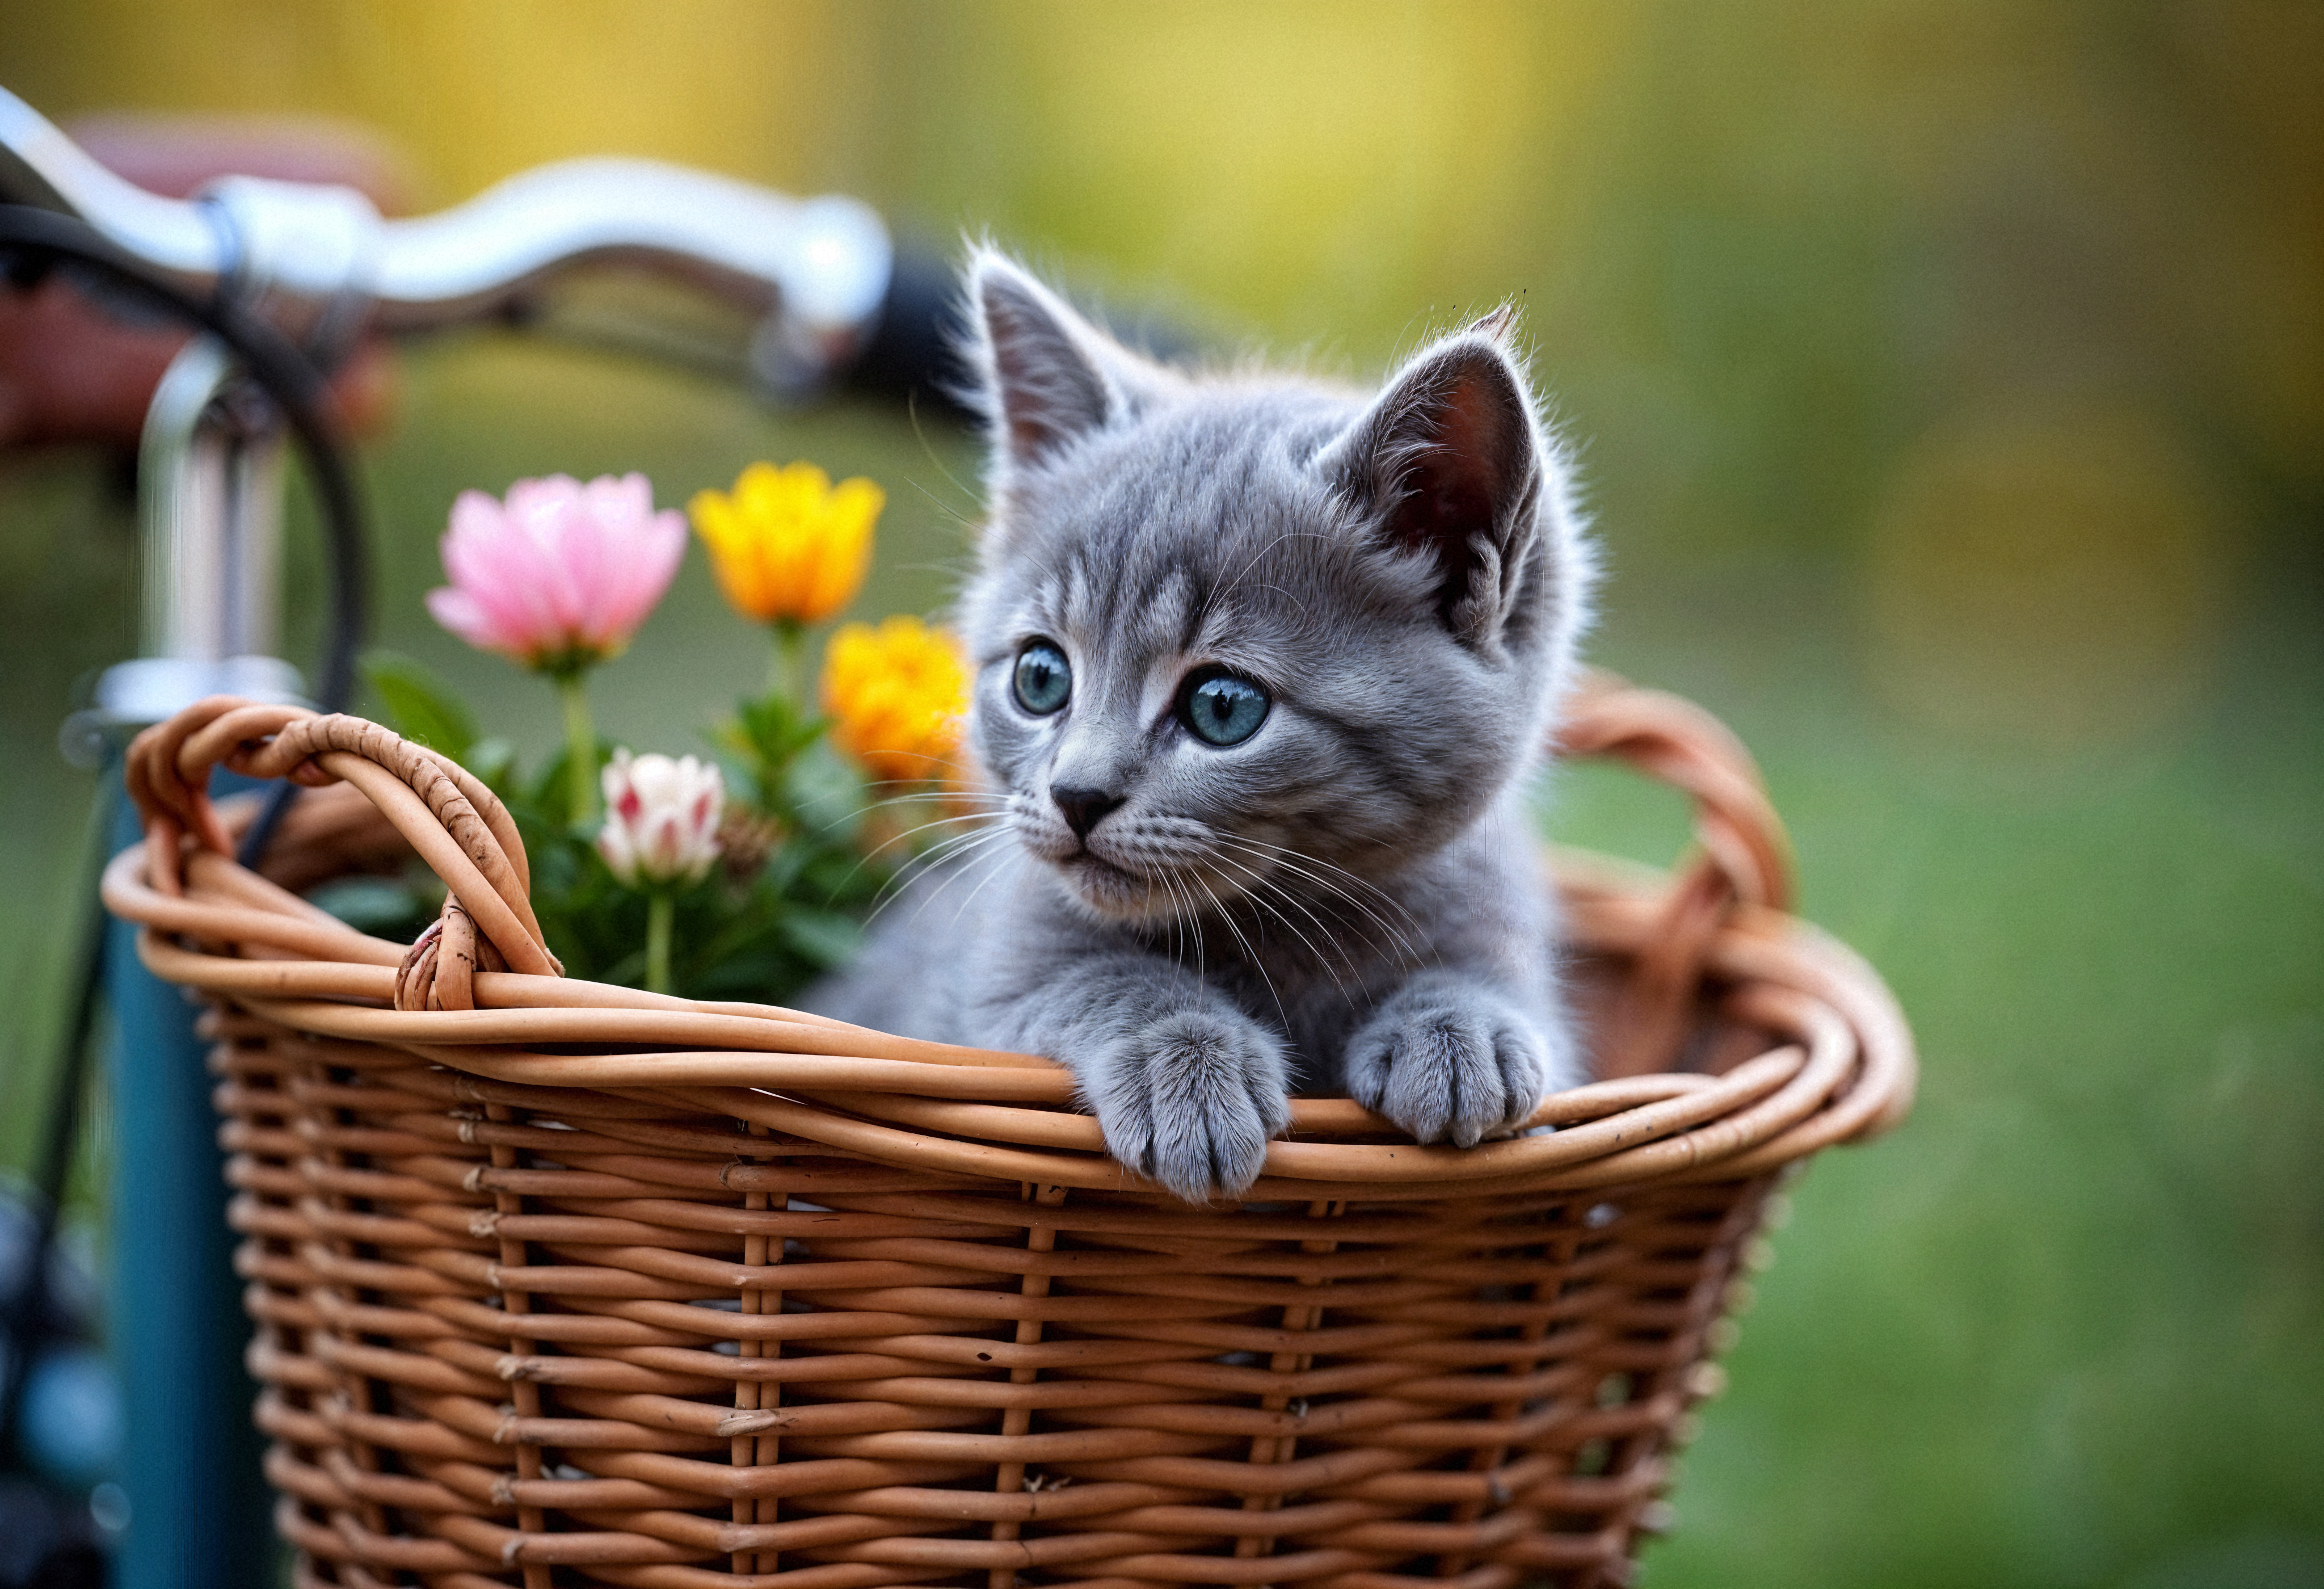
\includegraphics[width=1.0\textwidth, angle=0]{kotek.jpg}
\end{frame}

\begin{frame}
\centering
\frametitle{Skąd się pojawiły na ziemi koty i kotki}
\begin{columns}
\begin{column}{0.5\textwidth}
\begin{itemize}
\item Evolucja
\end{itemize}
Najbardziej prawdobodobnie znane nam koty domowe wyewolułowały z gatunków kotowatych jak tygrys czy lew po tym jak zaczeły żyć z ludźmi i przystosowały się do ludzi, dzięki czemu bardziej opłacało się im być słokdkimi niż zabujczymi
\includegraphics[height=0.4\textheight, angle=0]{tygrys.jpg}
\end{column}

\begin{column}{0.5\textwidth}
\begin{itemize}
\item wylazły z piekła
\end{itemize}
Inną teorią jest to że koty wylazły z piekła, zgadzało by się to z ich osobowością i dziwnymi umiejętnościami robienia rzeczy logicznie niemożliwych lub bez sensu oraz okazyjnymi zachowaniami jakby były opętane
\includegraphics[height=0.4\textheight, angle=0]{piekło.jpg}
\end{column}


\end{columns}
\end{frame}

\begin{frame}
\centering
\frametitle{Zalety posiadania kota}

Kiedy postanawiasz zająć się kotem wiążą się z tym oczywiście zalety jak i wady, zaczynając od bardziej pozytywnej części czyli zalet, zaletami posiadania kota są:
\begin{itemize}
\item brak samotności i posiadanie towarzysza
\item naturalny wpływ na zdrowie psychiczne wywołany głaskaniem kota i przebywaniem z nim
\item są śmieszne i slodkie
\item są dobrym żródłem kontentu na mediach społecznościowych
\item ciężko jest zaspać ponieważ są doskonałym budzikiem
\end{itemize}



\includegraphics[width=0.5\textwidth, angle=0]{zalety_kot.jpg}

\end{frame}


\begin{frame}
\centering
\frametitle{Wady posiadania kota}

Zalety zostały juz wspomniane teraz czas na wady posiadania kota, niestety nie ma nic bez wad a koty troche ich mają a tymi wadami są:
\begin{itemize}
\item sprzątanie po nich
\item nauczenie ich jak korzystać z kuwet i czego nie robić
\item wymagają atencji więc żadko masz spokuj
\item żyją krócej od ciebie
\item ciężko jest je oduczyć zaznaczania terenu
\item drapiom co mogą ściany, ciebie, krzesła oraz praktycznie wszystko inne co mogą
\item ciężko jest zabarykadować lub zamknąć miejsca do których nie chcesz żeby wchodziły

\end{itemize}


\includegraphics[width=0.5\textwidth, angle=0]{wady_kot.jpg}
\end{frame}

\begin{frame}
\centering
\frametitle{Zalety posiadania kotka}

Zalety i wady Kota już omówiłem teraz czas na zalety i wady kotków zaczynając od zalet będących:
\begin{itemize}
\item są mega słodkie ale tak naprawde słodkie
\item są małe i mają mały obszar poruszania się przez co łatwo je pilnować
\item opiekowanie się małom słodkom istotką ma dobry wpływ na psychike normalnego człowieka
\item zdobywa się dużo słokdich zdjęć i chwalenie się nimi jest naprawde przyjemne i daje łatwy teamat do rozmowy z ludźmi
\item nie czujesz się samotny w końcu masz kotka

\end{itemize}


\includegraphics[width=0.5\textwidth, angle=0]{zalety_kotek.jpg}
\end{frame}


\begin{frame}
\centering
\frametitle{Wady posiadania kotka}
\begin{columns}
\begin{column}{0.7\textwidth}
Wady posiadania kotka są głównie związane z tym że jest mały,młody i musisz nauczyć się jak obchodzić się z nim oraz go co może a czego nie może. Gdyby wymienić te wady to były by to: 
\begin{itemize}
\item kotek w końcu stanie się kotem
\item są małe i delikatne więc trzeba je pilnować
\item trzeba zrobić sporo wstępnych badań i szczepień
\item nie możesz o nim zapomnieć i zostawić go samego na zbyt dlugo
\item trzeba wszystkiego ich uczyć czyli jak używać kuwet, żeby nie drapały, żeby nie gryzły, gdzie mogą wejść a gdzie nie oraz że powinny aktualnie używać kuwet
\item ciężko się ich szuka jak nagle się ukryją w dziwnym miejscu

\end{itemize}
\end{column}

\begin{column}{0.3\textwidth}
\includegraphics[height=0.5\textheight, angle=0]{wady_kotek.jpg}
\end{column}
\end{columns}
\end{frame}

\begin{frame}
\centering
\frametitle{Podsumowanie na koniec}
Koty i kotki są inne z powodu róznic które pojawiają się podczas dorastania, niektóre rzeczy pozostają takie same a inne zmieniają się całkowicie. Ważne jest też pamiętać że każy kot czy kotek jest inny, kiedy większość staje się aktywna dopiero w nocy to też są koty co lubią dzień i śpią w nocy, są też koty co nie lubią głaskania i takie co muszą być głaskane przynajmniej 3 godziny. Według mnie osobiście jeśli ma sie czas i pieniadze na jedzenie warto mieć kota lub kotka, to po prostu przyjemne mieć taką mała istotke biegającą po domu i od czasu do czasu irytującą cię, to po prostu dodaje kolorów do życia.

\end{frame}

\begin{frame}
\setbeamertemplate{itemize items}[circle]
\frametitle{Żródła}
\begin{itemize}
\item \small https://redro.pl/fototapeta-niebieski-kot-brytyjski-nosi-okulary-lezace-na-ksiazki,63350960
\item https://www.karusek.com.pl/poradnik/koty-vs-fizyka/
\item https://pl.freepik.com/darmowe-zdjecie-wektory/slodki-kotek#uuid=2db6d84b-4199-4516-b354-f4e1d785f4d0
\item https://fajnepodroze.pl/tygrysy-ciekawostki-informacje-fakty/
\item https://www.ziarnko-gorczycy.pl/index.php/slowo-boze/dobre-slowo/950-684-pieklo-w-umysle-ludzkim
\item https://gazetalubuska.pl/wielka-galeria-kotow-zobaczcie-przeurocze-i-zabawne-zdjecia-pupili-naszych-czytelnikow/ar/c15-14946550
\item https://www.koty.pl/zachowanie-kota/kot-zrzuca-rzeczy-ze-stolu
\item https://lodz.pl/artykul/schronisko-w-lodzi-slodki-kociak-isio-szuka-domu-i-prawdziwego-przyjaciela-53278/
\item \small https://www.reddit.com/r/cat/comments/147gxx4/angry_cats/?tl=pl
\end{itemize}

\end{frame}

\begin{frame}
\centering
\huge Dziękuje za uwagę
\end{frame}

\end{document}

